%----------------------------------------------------------------------------------------
%	PAQUETES Y OTRAS COSAS DE CONFIGURACION
%----------------------------------------------------------------------------------------
%\documentclass[a4paper,man,natbib,scrbook]{apa6}
\documentclass[12pt]{article}

% esto es una prueba de comment
\usepackage[spanish]{babel}
\usepackage[utf8x]{inputenc}
\usepackage{graphicx}
%\usepackage[colorinlistoftodos]{todonotes} %PAQUETE QUE FALLA JULIO
\usepackage[bottom]{footmisc}
%\usepackage{blindtext} %PAQUETE QUE FALLA JULIO
\usepackage{caption}
\graphicspath{ {images/} }
%\graphicspath{{/home/cursoredes/images/}}
\usepackage{fancyhdr}
\usepackage{enumitem}
\usepackage{hyperref} %INDICE CON VINCULOS
\usepackage{csquotes}


%----------------------------------------------------------------------------------------
%	PAGE HEADERS
%----------------------------------------------------------------------------------------
\setlength{\headheight}{15pt}

\pagestyle{fancy}
\renewcommand{\sectionmark}[1]{ \markright{#1} }

% L=left, R=right, E=even, O=odd

\fancyhf{}
\fancyhead[LE,RO]{\thepage} %Numero pagina
\fancyhead[RE]{\textit{ \nouppercase{\leftmark}} }
\fancyhead[LO]{\textit{ \nouppercase{\rightmark}} }

\fancypagestyle{plain}{ 
  \fancyhf{} 
  \renewcommand{\headrulewidth}{0pt} 
  \renewcommand{\footrulewidth}{0pt}
}
%------------------------------------------------
%
%------------------------------------------------

\begin{document}

\begin{titlepage}

\newcommand{\HRule}{\rule{\linewidth}{0.5mm}} 

\center % Centra todo
 
 
%----------------------------------------------------------------------------------------
%	LOGO SECCION
%----------------------------------------------------------------------------------------

\textsc{\LARGE Universidad Complutense de Madrid}\\[0.1cm] % Universidad

\begin{center}
	\centering
	
\includegraphics[width=0.5\textwidth]{logo}
\end{center}
 
 
%----------------------------------------------------------------------------------------
%	HEADING SECCION
%----------------------------------------------------------------------------------------

\textsc{\LARGE Grupo 4}\\[0.1cm] % Grupo
%\textsc{\Large Heading 1}\\[0.5cm] % Heading mayor
%\textsc{\large Heading 2}\\[0.5cm] % Heading menor

%\textsc{\LARGE Grupo 4}\\[1cm]

%----------------------------------------------------------------------------------------
%	TITULO SECCION
%----------------------------------------------------------------------------------------

\HRule \\[0.4cm]
{ \huge \bfseries HITO 3: }\\[0.4cm] % Titulo
{ \huge \bfseries FRAMEWORK DE DISEÑO }\\[0.2cm] % Titulo
\HRule \\[1.2cm]
 
%----------------------------------------------------------------------------------------
%	AUTHOR SECTION
%----------------------------------------------------------------------------------------

\begin{minipage}{0.4\textwidth}
\begin{flushleft} \large
\emph{Autores:}\\
Ángel \textsc{Cruz} \\ %Nombres
Julio \textsc{de la Cruz} \\
Eduardo \textsc{Alcober}\\
Sergio \textsc{Gómez}\\
Isauro \textsc{López}\\
Darío \textsc{Gallegos}
\end{flushleft}
\end{minipage}
\begin{minipage}{0.4\textwidth}
\begin{flushright} \large
\emph{Profesor:} \\
Antonio \textsc{Sánchez} % NOMBRE PROFESOR
\end{flushright}
\end{minipage}\\[0.66cm]
%----------------------------------------------------------------------------------------
%	FECHA SECCION
%----------------------------------------------------------------------------------------
{\large 11 de noviembre de 2018}\\[0.5cm] % Fecha

%---------------------------------------------------------------------------------------
%	CONTENIDO
%----------------------------------------------------------------------------------------

\vfill % Rellenar el resto con espacio en blanco

\end{titlepage}


%\maketitle
%\footnotetext{EJEMPLO DE NOTA A PIE DE PAGINA}

\tableofcontents % Indice de contenidos
\newpage

%----------------------------------------------------------------------------------------
%	INTRODUCCION
%----------------------------------------------------------------------------------------

\section{Introducción}

Estamos siendo fieles a la esencia del proceso DGO: Diseño guiado por objetivos, por lo que nuestra prioridad hasta ahora ha sido detectar las metas que el usuario persigue al usar nuestro sistema. Hasta ahora hemos sido bastante abiertos a la hora de integrar o aceptar las funciones que hemos extraído de las entrevistas convirtiéndose en requisitos que pueden automatizar en cierta manera el uso de la biblioteca, pero a partir de este momento nos vamos a centrar en las siguientes funcionalidades básicas, con vistas a llegar a una definición final del sistema interactivo que nos dé tiempo a desarrollar en el trascurso de la asignatura:

\begin{itemize}

\item \textbf{Reserva de puestos en la biblioteca (inspirada en la aplicación car2go, es decir, con 10 minutos de reserva para evitar exceso de puestos reservados no ocupados, sin dejar de ofrecer la función)}
\item \textbf{Exploración del catálogo de la biblioteca María Zambrano/Integración con CISNE}
\item \textbf{Funcionalidad de Check in / Check out de los usuarios que permita un control de los puestos ocupados en la biblioteca, la renovación de una reserva, así como pausarla por 5-10 minutos. Planteamos que haya un periodo ventana o de adaptacion donde el personal de la biblioteca se encargue de "sentar" a las personas que no tienen la aplicacion y gestionar su reserva.}

\end{itemize}

\section{Alcance del hito}
Ya que la faceta más novedosa de nuestra aplicación se desarrolla en el lado del estudiante, por las diversas funcionalidades que hemos incluido, hemos decidido centrarnos en el diseño de esta vista, en vez de el acceso de administración/gestión que utilizaría el personal de la biblioteca.

Se ha descartado la opción de reserva de libros ya que supondría la introducción de un departamento de transporte de éstos entre bibliotecas de la UCM con su consiguiente impacto económico.

Respecto al sistema de Check in en los puestos de la biblioteca, hemos contemplado dos opciones, con los siguientes inconvenientes:

\begin{itemize}
\item \textbf{Código QR en el puesto - Scan vía terminal móvil con cámara: Esta opción sería bastante asequible, pero aporta la posibilidad del deterioro de los QR y la necesidad de su renovación periódica (relativamente barata - cambiar pegatina).}

\item \textbf{Generación de QR en la App. - Scanner en el puesto: El QR incluye el tiempo de reserva seleccionado por el usuario. Esta opción es la más cara por la instalación de un servicio de check in por mesa. Ante esta opción se plantea la instalación de 2 o 3 máquinas autónomas de escaneo de códigos por sala donde cada usuario puede hacer check-in. PENDIENTE DUDA PROFESOR CUÁL IMPLEMENTAR}
\end{itemize}

Por comodidad y coherencia con el sistema de la UCM hemos decidido que este servicio vaya asociado a la cuenta de los estudiantes UCM como un servicio más del Campus Virtual, no permitiendo alta de usuarios externos que al no tener carnet Complutense no podrían hacer uso de las instalaciones.

Es también un punto muy importante a decidir si se llega a implantar el sistema cómo hacer la gestión de los puestos de los usuarios “de a pié”, que la utilizan del modo tradicional de asistencia sin reserva previa o incluso sin terminal móvil. Nosotros proponemos que la aplicación pude estar instalada en algunos ordenadores en la biblioteca donde estos usuarios podrían hacer sus gestiones, o que el personal de la biblioteca sea el encargado de asignar y gestionar desde su puesto de control la entrada/salida de este tipo de usuarios.



\section{Organización y reparto de tareas}
En busca de buenas ideas y de aportar lo mejor de cada miembro del equipo, comenzamos con un brainstorming de mockups. Este inicio nos ha permitido plantearnos de forma profunda el flujo de navegación sobre la interfaz, acercar posturas en cuanto al tratamiento de las funciones principales y ante la explosión de material, hemos escogido las mejores ideas para agrupar y presentar las funciones de la aplicación. A partir de este análisis hemos definido los keypaths 


\begin{itemize}

\item \textbf{Documentación}: Permite a los miembros de nuestro grupo disponer de las aptitudes y conocimientos necesarios para el siguiente hito.

\item \textbf{Correcciones del hito anterior}: Tras recibir el feedback del anterior hito, es
necesario aplicar las correcciones pertinentes para la entrega final.

\item \textbf{Diseño de un boceto conceptual}: Consiste en elaborar un diseño preliminar que nos permita asentar las bases de cómo va a ser el producto final. Es la parte más creativa del proceso ya que un problema se puede resolver de muchas maneras, y  es aquí donde la mente creativa piensa en distintas soluciones y plantea múltiples propuestas. 

\item \textbf{Escenarios keypath}: Revisando los escenarios del hito anterior, narramos el proceso de uso de la aplicación. El objetivo es que sea más fácil elaborar un primer boceto; nos permite definir por ejemplo el número de mockups de la aplicación, componentes de cada una de ellas o como interactúan entre sí.

\item \textbf{Escenarios de validación}: Es complicado definir cúal será el flujo de interación, si todas las interacciones del usuario estarán cubiertas, y cuando ocurra algo imprevisto. Recopilado los casos del brainstorming más la experiencia de los propios miembros del equipo con otras aplicaciones y su propia interpretación se ha intentado esclarecer cómo reaccionará la aplicación ante situaciones inesperadas. 

\item \textbf{Documento de elementos}: Consiste en definir la forma de la aplicación, la postura con la que vamos a afrontar el desarrollo y los elementos con los que vamos a trabajar como por ejemplo el tipo de datos.

\item \textbf{Mockups de la aplicación}: Cada miembro del equipo debe crear de seis a ocho mockups según la visión que tenga sobre la aplicación. Los requisitos mínimos que han de contener son los del boceto conceptual. Una vez realizados se ponen en común y se eligen las mejores soluciones para cada mockup.

\item \textbf{Un diseño final}: Nos encargamos de refinar la interfaz y corregir los fallos restantes para elaborar del diseño final.


\begin{center}
	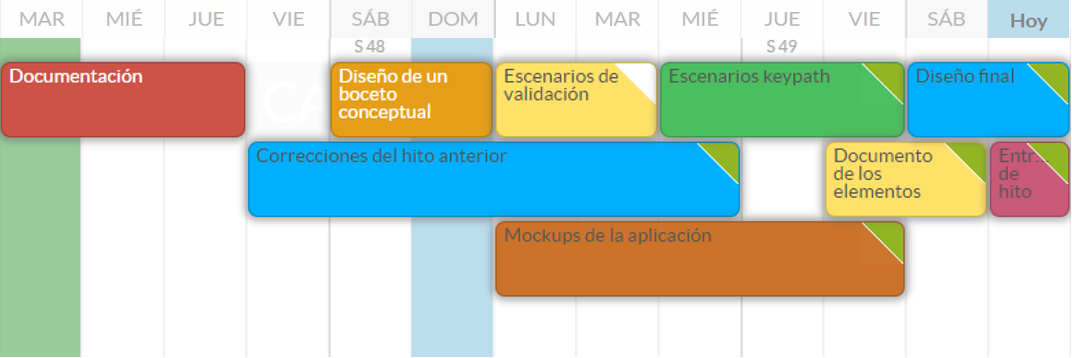
\includegraphics[width=1\textwidth]{planificacionHito3.png}
		\captionof{figure}{Planificación de tareas \href{https://drive.google.com/open?id=1CvTkgm0EXWupOtpI0MY0mefCv1vXhViW}{(PDF: planificacionHito3.pdf)} }
\end{center}
\phantom{10}

Los miembros del grupo trabajaremos con un esquema descentralizado controlado, donde las tareas asignadas a cada miembro podrán ser intercambiadas hacia otro; contemplando alguna incidencia si fuera el caso. Luego los miembros del grupo repasamos en profundidad todos los documentos a entregar.

\end{itemize}
\newpage

%----------------------------------------------------------------------------------------
%	DEFINIR LOS PUNTOS DE VISTA QUE USAMOS PARA GENERAR EL PROTOTIPO
%----------------------------------------------------------------------------------------

\section{Definiciones del  framework  de iteracción}

\subsection{Definición del factor de forma}
\begin{itemize}

\item Como se aprecia en los escenarios de contexto los estudiantes van a utilizar la aplicación tanto dentro como de camino a la biblioteca, generalmente en un terminal móvil (Android o AppleIOS) aunque al ser un servicio (teóricamente)

\item Se puede instalar la aplicación en un dispositivo tactil autónomo para que los estudiantes “de a pié” sin aplicación puedan hacer su auto-reserva (irrelevante para nuestro desarrollo)

\end{itemize}
\subsection{Definición de la postura}
\begin{itemize}

\item Consideramos que la postura del usuario ante nuestra aplicación es temporal ante todas sus funcionalidades ya que las operaciones no deben alargarse demasiado. A este respecto hemos incluido algunos iconos que directamente en el “Panel de Usuario” (Dashboard) indican con un color si el servicio no está disponible y la razón mediante un pop-up.

\end{itemize}
\subsection{Definicion del método de entrada}
\begin{itemize}

\item El método de entrada va a ser generalmente táctil, pudiendo ser fácilmente adaptable a su uso con ratón común.

\end{itemize}
\subsection{Definición de los elementos de datos y funcionales }
    \subsubsection{Elementos de datos}
    \subsubsection{Elementos funcionales}
\newpage
\section{Esquema del framework de interacción}

\begin{itemize}
\item Login - servicio asociado a cuenta UCM
\begin{itemize}
\item Tutorial en primer login
\item Recordar cuenta
\item Icono de Idioma (cambiar)
\end{itemize}
\item Dashboard personal (perfil) (minimalista, Shazam + Bottom Menu + Top Notifications)
\begin{itemize}
\item Avisos/Notificaciones sobre devoluciones o Alertas del sistema (Top)
\begin{itemize}
\item Notificación tiempo de reserva terminando (también desde fuera de la app)
\item Vencimiento de reserva de libros
\item Libro que quieres reservar está disponible

\end{itemize}

\item Mi lista (arriba junto a notificación, Corazón)

\item Settings (arriba junto a notificación, Tuerca) (ToS gordo, enlace web a la biblio)

\begin{itemize}
\item Modo Noche
\item Notificaciones Si/No
\item Notificaciones Vibración/Sonido
\item Vaciar Historial de Búsqueda
\item Informar de un problema (le metemos un mensajito de “será solucionado pronto” y jamás lo miramos)
\item Cambiar Idioma

\end{itemize}

\item Acceso a búsqueda de libros (Bottom)

\begin{itemize}
\item Búsqueda (cuadro)
\item Last Borrowings (slide)
\begin{itemize}
\item Ficha de Libro ejemplar biblioteca

\end{itemize}

\end{itemize}

\item Acceso a los asientos para reserva (Bottom)

\begin{itemize}
\item Listado de salas de biblioteca
\begin{itemize}
\item Sala concreta: Mapa conceptual con luces rojas y verdes en función de disponibilidad

\end{itemize}
\end{itemize}

\item Check in sitio libre (Único, desaparece una vez escaneas el QR, reaparece en modo espera)

\item Check out (activado si procede). (Abandonar puesto definitivamente y liberarlo) (Una vez escaneado el QR aparece)
\item Opción “poner en espera” 10-15m (activada si procede). (Una vez escaneado el QR aparece)

\item Ampliar tiempo de reserva (activado si procede) (Una vez escaneado el QR aparece)


\end{itemize}

\item Información de la Biblioteca

\end{itemize}





\newpage
%----------------------------------------------------------------------------------------
%	BOCETOS DEL FRAMEWORK DE ITERACCIÓN
%----------------------------------------------------------------------------------------
\section{Bocetos del framework de iteracción}

Estos bocetos estan en myBalsamiq (en la carpeta del grupo 4) y en una carpeta auxiliar que adjuntamos con la memoria de este hito.

%--------------------------------------------------------------------------------------------
%   ESCENARIOS KEYPATH
%--------------------------------------------------------------------------------------------
\section{Escenarios keypath}

Partiendo de los escenarios del hito anterior, narramos el proceso de uso de la aplicación para caso. Por ejemplo, Alex quiere reservar una mesa para estudiar. Enciende su movil y accede a la aplicación. Al ser la primera vez que la usa, debe introducir su cuenta de ucm y contraseñas. Las proximas veces que entre no será necesario. Pulsa en el boton de enter y va a la pagina princial. En el meú inferior pulsa el item puesto libre el cual ... 
 \\
 \\
\textbf{\underline{Login}} \\
 \\
Al iniciar la aplicación se muestra la pantalla de login (Figura 2). El usuario deberá introducir en los campos ‘Usuario’ y ‘Contraseña’ su cuenta de correo UCM y su contraseña de la misma respectivamente. A continuación, el usuario debe pulsar en el botón ‘Entrar’, su correo y cuenta serán verificadas y si son correctas se le llevará a la siguiente pantalla. Si ya tiene la sesión UCM iniciada en su dispositivo esta pantalla se omite. Una vez iniciada la sesión, se muestra la pantalla principal de la aplicación. (Figura 3)\\

\begin{figure}[!h]
\centering
\minipage{0.46\textwidth}
	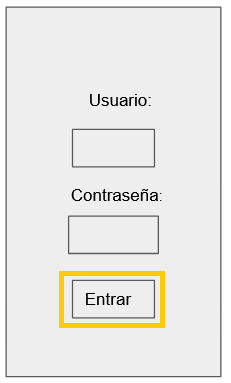
\includegraphics[width=0.5\textwidth]{login.png} 
	\captionof{figure}{}
\endminipage
\minipage{0.46\textwidth}
	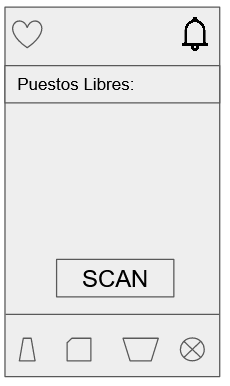
\includegraphics[width=0.5\textwidth]{dashboard.png} 
	\captionof{figure}{}
\endminipage
\end{figure}

\textbf{\underline{Ver notificaciones}} \\
\\
Para ver las notificaciones el usuario deberá pulsar el icono de la campana, esto desplegará un pop-up con la lista de notificaciones. (Figura 4)
El usuario puede borrar las notificaciones deslizando el dedo de derecha a izquierda sobre la notificación que desee eliminar. (Figura 6)\\

\begin{figure}[!h]
\centering
\minipage{0.46\textwidth}
	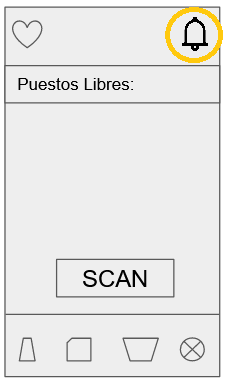
\includegraphics[width=0.5\textwidth]{notificaciones1.png} 
	\captionof{figure}{}
\endminipage
\minipage{0.46\textwidth}
	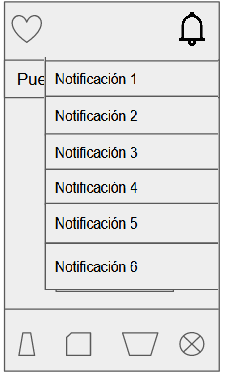
\includegraphics[width=0.5\textwidth]{notificaciones2.png} 
	\captionof{figure}{}
\endminipage
\end{figure}
\begin{figure}[!h]
\centering
\minipage{0.46\textwidth}
	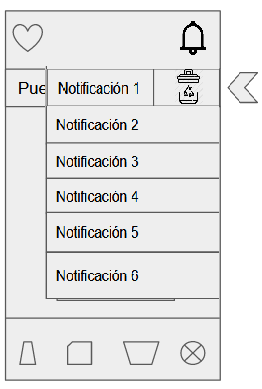
\includegraphics[width=0.5\textwidth]{notificaciones3.png} 
	\captionof{figure}{}
\endminipage
\end{figure}

\newpage
\textbf{\underline{Búsqueda de libros}} \\
\\
El usuario puede acceder a la pantalla de búsqueda de libros pulsando sobre el segundo icono de la barra de menú. (Figura 7) El usuario puede a continuación; buscar y filtrar sus búsquedas con los criterios de los que dispone.

La lista resultante de libros puede ser visualizada en la parte central de la pantalla y permite navegar por la lista con un scroll horizontal que maneja el usuario con el dedo. (Figura 8)\\

\begin{figure}[!h]
\centering
\minipage{0.42\textwidth}
	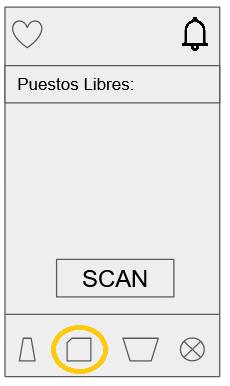
\includegraphics[width=0.5\textwidth]{busquedaLibros1.png} 
	\captionof{figure}{}
\endminipage
\minipage{0.58\textwidth}
	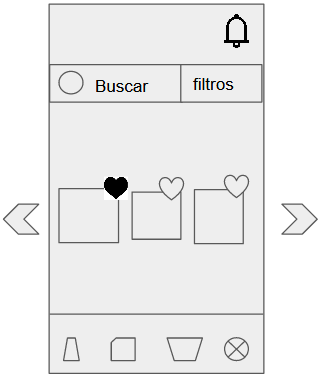
\includegraphics[width=0.5\textwidth]{busquedaLibros2.png} 
	\captionof{figure}{}
\endminipage
\end{figure}

\textbf{\underline{Búsqueda de sitio}} \\
\\
El usuario puede acceder a la pantalla de búsqueda de sitios pulsando sobre el tercer icono de la barra de menú. (Figura 9) 

A continuación se le muestra al usuario información sobre la biblioteca que le puede ser de interés, en nuestro caso, para acceder y visualizar los sitios, hemos de pulsar sobre el mapa de la biblioteca. (Figura 10) 

Se nos mostrará un mapa general de las 4 zonas de la biblioteca, cada una con un indicativo sobre cuántos sitios libres quedan. Para buscar un sitio concreto, seleccionamos la zona deseada. (Figura 11)

A continuación se muestra un mapa concreto de la sala indicada. Seleccionamos el asiento libre que queramos.(Figura 12) 

La aplicación mostrará un camino desde la entrada de la sala para llegar a nuestro asiento. (Figura 13)\\

\begin{figure}
\centering
\minipage{0.45\textwidth}
	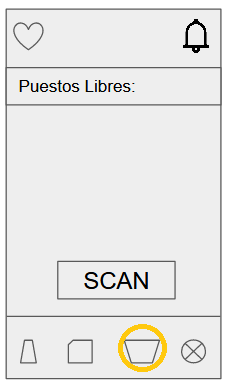
\includegraphics[width=0.45\textwidth]{mapa.png} 
	\captionof{figure}{}
\endminipage
\minipage{0.45\textwidth}
	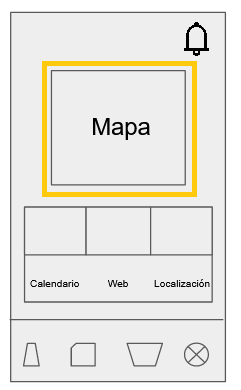
\includegraphics[width=0.45\textwidth]{mapa1.png} 
	\captionof{figure}{}
\endminipage

\medskip

\minipage{0.45\textwidth}
	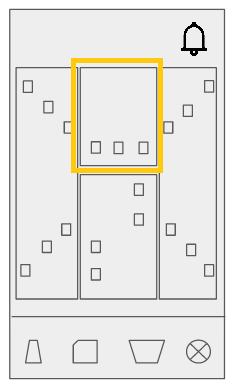
\includegraphics[width=0.45\textwidth]{mapa2.png} 
	\captionof{figure}{}
\endminipage
\minipage{0.45\textwidth}
	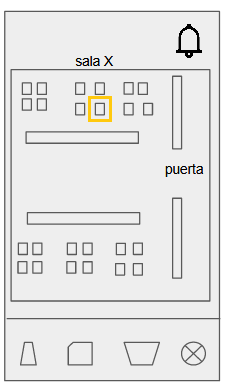
\includegraphics[width=0.45\textwidth]{mapa3.png} 
	\captionof{figure}{}
\endminipage

\medskip

\minipage{0.45\textwidth}
	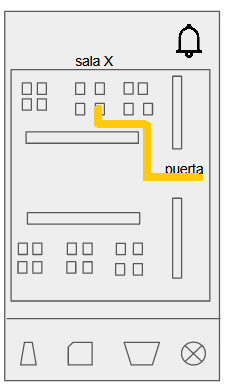
\includegraphics[width=0.45\textwidth]{mapa4.png} 
	\captionof{figure}{}
\endminipage
\end{figure}

\newpage
\textbf{\underline{Reserva de sitio}} \\
\\
Una vez llegado al sitio, el usuario puede escanear el código QR del sitio para realizar la reserva.

Para ello, primero debe pulsar en el botón ‘SCAN’ del dashboard. (Figura 14) La cámara se encenderá para reconocer el QR. (Figura 14) Una vez reconocido exitosamente el QR la aplicación confirma la reserva y exige confirmación por parte del usuario. (Figura 16) La reserva se ha completado, el usuario es redirigido a un nuevo dashboard en el que puede gestionar su reserva activa.(Figura 17)\\

\begin{figure}[!h]
\centering

\minipage{0.46\textwidth}
	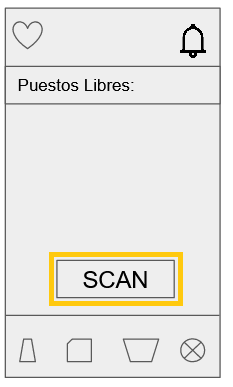
\includegraphics[width=0.5\textwidth]{reservaSitio1.png} 
	\captionof{figure}{}
\endminipage
\minipage{0.46\textwidth}
	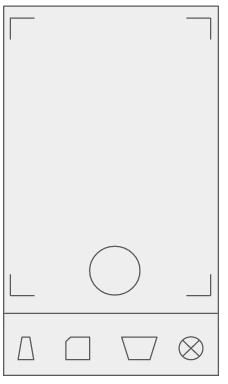
\includegraphics[width=0.5\textwidth]{reservaSitio2.png} 
	\captionof{figure}{}
\endminipage

\medskip

\centering
\minipage{0.46\textwidth}
	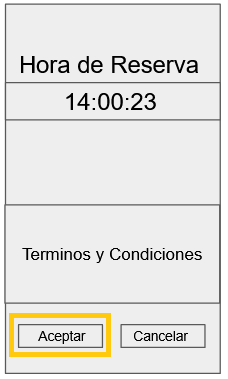
\includegraphics[width=0.5\textwidth]{reservaSitio3.png} 
	\captionof{figure}{}
\endminipage
\minipage{0.46\textwidth}
	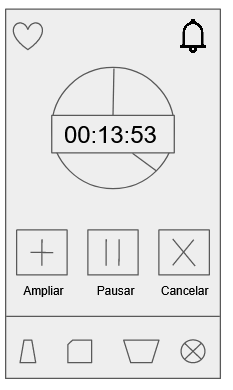
\includegraphics[width=0.5\textwidth]{reservaSitio4.png} 
	\captionof{figure}{}
\endminipage
\end{figure}

\newpage
%--------------------------------------------------------------------------------------------
%   ESCENARIOS VALIDACIÓN
%--------------------------------------------------------------------------------------------
\section{Escenarios de validación}
En términos generales, es muy difícil generar un flujo de mockups los suficientemente amplio como para estimar todas las interacciones del usuario, y menos aún, las interacciones no previstas. Se han recopilado los casos a partir de un brainstorming basado en la experiencia de los propios miembros del equipo con otras aplicaciones y su propia interpretación de los flujos de los mockups en los supuestos escenarios de validación.
\\
\\
\\
\textbf{¿Usuario incorrecto, contraseña incorrecta?}
A parte de reenviar al usuario al formulario de login y marcar en rojo un aviso de
error de “usuario/contraseña”, independientemente de que ese mail esté registrado o no.
\\
\\
\textbf{¿Desconexión del usuario por falta de cobertura?}
Este caso tiene más riesgo sobre todo dentro de edificios, ya que los dispositivos pueden sufrir desconexiones interrumpiendo el servicio de la aplicación. En estos casos, el usuario llegaría a una vista no alcanzable mediante interacción normal de la aplicación. 
Se le mostrará un mensaje solicitando que obtenga una conexión de datos para retomar el funcionamiento normal de la aplicación.
\\
\\
\textbf{¿Cerrar la aplicación cuando está creándose una reserva?}
Al igual que ocurre con los formularios de registro, un cierre en la aplicación conlleva a la cancelación de la reserva.
\\
\\
\textbf{¿Reconexión?}
El proceso de reconexión de la aplicación abierta, deben reubicar al usuario en la
vista en la que se encontraba antes de perder la conexión, si estaba en un periodo
específico de una reserva, y al reconectarse está ya en otra etapa, el ventana del usuario será actualizada a la nueva vista.
\\
\\
\textbf{El usuario busca un libro que no está en la biblioteca.}
La búsqueda no devuelve resultados.
\\
\\
\textbf{El usuario vuelve pulsa el botón de añadir a la lista de favoritos un libro que ya está en la lista.}
El libro es eliminado de la lista de favoritos.
\\
\\
\textbf{El usuario selecciona una zona sin sitios libres para buscar sitio.}
Aparece un mensaje de error indicando que no hay sitios disponibles e indicando la hora en la que podría liberarse el siguiente asiento.
\\
\\
\textbf{El usuario no recuerda la contraseña.}
Al pulsar en el enlace en la pantalla de login “¿has olvidado tu contraseña?” es redireccionado a la página web del servicio de correo UCM.
\\
\\
\textbf{El usuario selecciona el icono de idioma en la pantalla de login.}
Una lista con las distintas opciones de idiomas aparece, el usuario puede seleccionar si cambiar el idioma o no pulsando en retroceder o en el icono de idioma correspondiente.
\\
\\
\textbf{El usuario tiene la pantalla apagada cuando el tiempo de reserva está a punto de expirar.}
El usuario puede configurar en el menú de opciones con cuánto tiempo y de qué modo se le notifica, por defecto, el móvil empezará a vibrar cuando queden 10 minutos para que expire la reserva.
\\
\\
\textbf{El usuario cierra la aplicación cuando tiene una reserva activa.}
La aplicación se recupera cuando se abra de nuevo, si no la vuelve a abrir, esta permanece en 2º plano y notificará al usuario cuando su reserva esté a punto de expirar.
\\
\\
\textbf{El usuario cierra la aplicación cuando tiene una reserva activa pero la configuración de su móvil no permite a nuestra aplicación ejecutar en segundo plano.}
El usuario podrá permanecer en su asiento tanto tiempo como tiempo de reserva quedase, no obstante ese comportamiento inflige los términos de condiciones de uso.
\\
\\
\textbf{El usuario no se encuentra en la biblioteca y abre la cámara para reservar un asiento desde otro sitio haciendo uso de una copia del QR de la mesa.}
Este comportamiento inflige los términos de condiciones de uso, esta situación no está controlada y si un sitio aparece ocupado y está vacía, otro usuario puede notificarlo al bibliotecario. El bibliotecario puede entonces sancionar al usuario.
\\
\\
\textbf{Un no usuario de la aplicación quiere hacer uso de la biblioteca.}
El no usuario puede hacer uso de las instalaciones, esta situación será frecuente en un inicio pero sobre la que no se puede tener control, a menos que se tomen medidas que permitan saber qué sillas están siendo ocupadas.
\\
\\
\textbf{El usuario olvida cómo utilizar alguna pantalla u opción del proceso de reserva de sitios o búsqueda de libros.}
El la sección de opciones, el usuario tiene la opción de ver el tutorial de la sección que le interese.
\\
\\
\textbf{La cámara lee un QR no válido.}
Se le muestra al usuario un mensaje de error.
\\
\\
\textbf{El usuario busca un libro y sin querer, cambia de menú y navega al dashboard o a otro menú.}
El menú de búsqueda de libros recuerda el último estado en el que se encontraba para permitir al usuario recuperarse de errores.
\\
\\
\textbf{El usuario realiza reserva libros y olvida cuál es la fecha límite de devolución.}
El sistema de notificaciones, al estar enlazado con la cuenta UCM, notifica al usuario sobre las fechas próximas en las que vencen sus pedidos.
\\
\\
\textbf{El usuario abre y cierra la aplicación con mucha frecuencia.}
Si el la configuración y el estado del dispositivo del usuario lo permiten, la cuenta ucm sigue enlazada al dispositivo, por lo que no es necesario hacer el proceso de login múltiples veces.


%--------------------------------------------------------------------------------------------
%   PROCESO ITERATIVO
%--------------------------------------------------------------------------------------------
\section{Proceso iterativo}

\textbf{1ª Iteración}:
Consideramos parte de esta iteración el diseño del flujo principal de la aplicación,
definido en los “mockups”. En ella nos centramos en plasmar qué pasos y qué funcionalidades debe tener la aplicación basándonos en los requisitos obtenidos en el hito anterior.
En el proceso del diseño de esta interfaz primitiva, se han ido realizando pequeñas
correcciones, botones mal ubicados o poco intuitivos principalmente.

\textbf{2ª Iteración}:
En esta etapa se diseñaron, de forma paralela, lo que podría interpretarse como la
primera implementación de lo obtenido en la primera iteración.
\begin{itemize}

\item El primer diseño fue hecho en Balsamiq de forma individual, un diseño por cada miembro del equipo, de forma rápida y con baja calidad. Se centra principalmente en portar, de una forma fiel, los esquemas e ideos de los bocetos.
\item El segundo diseño, hecho en papel, busca esto mismo, pero arriesgando un poco más su estilo con diseños redondeados más llamativos a la vista. Se centra en recalcar y facilitar “el camino más tomado”. Aquel que la gran mayoría de usuarios va a tomar.

\end{itemize}
\textbf{3ª Iteración}:
Finalmente, se ponen en común los dos diseños generados en la etapa anterior.
Aquellas ventanas en las que se necesite una estructura ordenada heredarán su forma del primero, mientras que aquellas que sean “de paso” y tengan una mayor libertad, seguirán las líneas del segundo diseño.


\end{document}

%COMENTAARIOS
% \todo[inline, color=green!40]{EJEMPLO DE COMENTARIO}

% PARA INCLUIR UNA FOTOGRAFIA:
%\begin{figure}
%\centering
%\includegraphics[width=0.5\textwidth]{~/DIRECCION/A/IMAGEN.jpg}
%\caption{\label{fig:imagen}DESCRIPCION.}
%\end{figure}

% \dots

% ENUMERACION:
%\begin{enumerate}
%\item Enumeracion 1
%\item Enumeracion 2
%\end{enumerate}

%\begin{itemize}
%\item PUNTO 1

% PARA INCLUIR UNA TABLA:
%\begin{table}[h] %LA h PARA INDICAR QUE LA TABLA NO SEA FLOATING
%\centering
%\begin{tabular}{l|r}
%Fila 0 \\\hline
%Fila 1 & Contenido 1 \\
%Fila 2 & Contenido 2
%\end{tabular}
%\caption{\label{tab:widgets}Ejemplo de tabla.}
%\end{table}

%\item PUNTO 2
%\end{itemize}

%\bibliography{BIBLIOGRAFIA}


